
\documentclass[journal]{IEEEtran}
\usepackage[section]{placeins}
\usepackage{blindtext}
\usepackage{graphicx}
\usepackage{caption}
\usepackage{amsmath}
\usepackage{hyperref}
\usepackage{mwe}
\usepackage{algorithm2e}


\ifCLASSINFOpdf
\else
\fi
\hyphenation{Dictionary Based Filtering}


\begin{document}
	%
	% paper title
	\title{Dictionary Based Filtering}
	
	\author{\thanks{Dr. Mehul Raval}\thanks{Mr. Vaibhav Joshi} 
		Group - 8\\
		Charvik Patel,~\IEEEmembership{1401079},
		Himanshu Budhia,~\IEEEmembership{1401039},\\
		Neel Puniwala,~\IEEEmembership{1401024}, 
		Maharsh Patel,~\IEEEmembership{1401109}}
	
	
	
	
	% make the title area
	\maketitle
	
	
	\begin{abstract}
		%\boldmath
		Digital image processing refers to the process of digital
		images by means of digital computer. The main application
		area in digital image processing is to enhance the pictorial
		data for human interpretation. In image some of
		the unwanted information is present that will be removed by
		several preprocessing techniques. Filtering helps to enhance
		the image by removing noise.Initially By creating Dictionary we will store two form of matrix.now when We add new image in dictionary we don't need to pass image from filter instead we will just Dictionary Learn form the Previous Dictionary and just map into.
		
	\end{abstract}
	\begin{IEEEkeywords}
		Dictionary Learning,Low-pass filter,Salt-Pepper Noise,Median filter
	\end{IEEEkeywords}
	
	
	\IEEEpeerreviewmaketitle
	
	
	
	\section{\textbf{Introduction}}
	Basically the idea of Dictionary based filtering is instead of doing classical convolution every time,we directly take de\textendash noise image from the dictionary using searching algorithm and time after time Learning of dictionary is also done by the same algorithm. We are planning to do low pass or high pass filtering to de\textendash noise the noisy image. Low pass filter is used to remove salt and paper noise while high pass filter is used to separate of edges.We use OpenCV libraries and Python libraries to implement the low pass filter and to create blocks of image.
	
	Initially we take some training and filter them by using classical convolution.Both filtered and non-filtered images are divided into blocks which are stored in a dictionary.In the dictionary the key is noisy part of the image and the value is filtered part of the image.
	
	\section{\textbf{Literature review}}
	\subsection{Sparse Dictionary Learning$^{[2]}$}
	Sparse dictionary learning is a representation learning
	method which aims at finding a sparse representation of the
	input data (also known as sparse coding) in the form of a
	linear combination of basic elements as well as those basic
	elements themselves. These elements are called atoms and they
	compose a dictionary. Atoms in the dictionary are not required
	to be orthogonal, and they may be an over-complete spanning
	set. This problem setup also allows the dimensionality of the
	signals being represented to be higher than the one of the
	signals being observed.
	
	One of the key principles of dictionary learning is that the
	dictionary has to be inferred from the input data. The emergence
	of sparse dictionary learning methods was stimulated
	by the fact that in signal processing one typically wants to
	represent the input data using as few components as possible.
	
	Different Algorithm for Sparse Dictionary Learning are as
	follow.
	\begin{enumerate}
		\item \textbf{K-SVD:}$^{[8]}$
		Applications that use sparse representation are many and include compression, regularization in inverse problems, feature extraction, and more.Sparsity in over-complete dictionaries is the basis for a wide variety of highly effective signal and image processing techniques.
		Model: Given a dictionary D and a signal y,
			$ \stackrel{min}{x}\parallel x \parallel_0 \hspace{0.5cm} s.t.\hspace{0.2cm} y=Dx $\\
				or\\
			$ \stackrel{min}{x}\parallel x \parallel_0 \hspace{0.5cm} s.t.\hspace{0.2cm} \parallel y-Dx \parallel_2\le \varepsilon $
			

		where,\\
		
		\textbf{$D \epsilon R^{n * K}$:}an overcomplete dictionary matrix \\
		\textbf{$y \epsilon R^n$}:a signal can be represented as a sparse linear
		combination of columns of D \\
		\textbf{$x \epsilon R^K$}:a vector contains the representation
		coefficients of the signal y.
		
		\textbf{Training Approach And Algorithm}
		
		Train the dictionary directly based on the given examples, optimizing w.r.t. sparsity and other desired properties.\\
			
		\textbf{Output:}\\
		\begin{minipage}{\linewidth}
			
			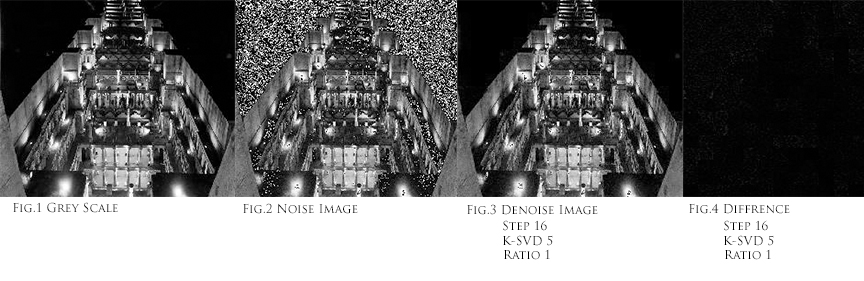
\includegraphics[width = 80mm,height=25mm]{KSVD.jpg}
			\captionof{figure}{ K-SVD - Step 16 - kSVD 5 - Ratio 1$^{[12]}$ \label{overflow}}
		\end{minipage} 
		\linebreak
		\item \textbf{Online dictionary learning$^{[3]}$:} 
		Many common approaches to sparse dictionary learning rely on the fact that the whole input data $X$ (or at least a large enough training dataset) is available for the algorithm. However, this might not be the case in the real-world scenario as the size of the input data might be too big to fit it into memory. The other case where this assumption can not be made is when the input data comes in a form of a stream. Such cases lie in the field of study of online learning which essentially suggests iteratively updating the model upon the new data points $x$ becoming available.\\
		A dictionary can be learned in an online manner the following way
		\begin{enumerate}
			\item for $t=1,2,3...T$
			\item Draw a new sample $x_t$
			\item Find a sparse coding using LARS
			\item Update dictionary using block-coordinate approach
		\end{enumerate}
	
		\textbf{Output:}\\
		\begin{minipage}{\linewidth}
			
			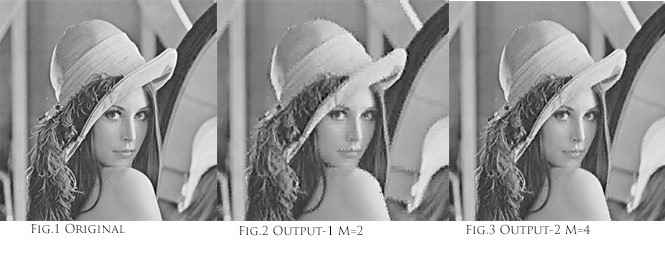
\includegraphics[width = 80mm,height=40mm]{OnlineDictionaryLearning.jpg}
			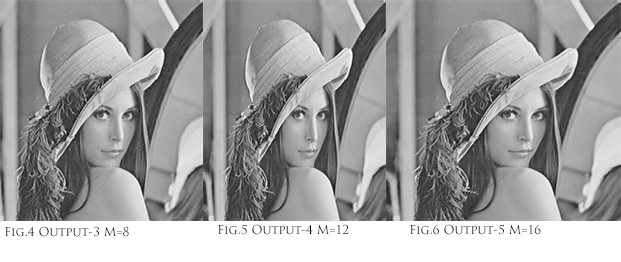
\includegraphics[width = 80mm,height=40mm]{OnlineDictionaryLearningCopy.jpg}
				
			\captionof{figure}{ On-line Dictionary Learning for m=2,4,8,12,16$^{[7]}$ \label{overflow}}
		\end{minipage} 
			
	\end{enumerate}
%	\section{\textbf{Flow of Implementation}}
%	\begin{algorithm}
%	First of all we have to take n x n training
%	image.\\
%		Create m x m blocks.\\
%		Create dictionary using blocks.\\
%		Dictionary:\\
%		\hspace{1cm}	 \textbf{Key} - Noisy image\\
%		\hspace{1cm}	 \textbf{value} - filtered image\\
%		Search algorithm\\
%			\eIf{Nearest Possible Match}{
%				Noisy Patch Replaced with this Image
 %   		}{
%			Add to Dictionary
%		}
%	return \textbf{Final Filtered Image}
	
%\end{algorithm}

\section{Our Own Approach for Dictionary Based Filtering}
\subsection{Input}
Salt-and-pepper noise is a form of noise sometimes seen
on images. It presents itself as sparsely occurring white and
black pixels. An effective noise reduction method for this type
of noise is a median filter. We take a set of images with salt and pepper noise present at random positions.
\subsection{Algorithm}
An effective noise reduction method for this type of noise is a median filter. Like the mean filter, the median filter considers each pixel in the image in turn and looks at its nearby neighbors to decide whether or not it is representative of its surroundings. Instead of simply replacing the pixel value with the mean of neighboring pixel values, it replaces it with the median of those values. The median is calculated by first sorting all the pixel values from the surrounding neighborhood into numerical order and then replacing the pixel being considered with the middle pixel value.
\begin{minipage}{\linewidth}
	\centering
	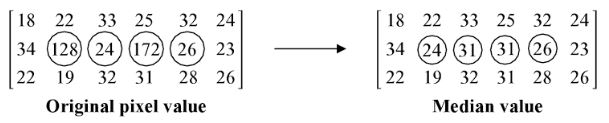
\includegraphics[width=80mm]{1}
	\captionof{figure}{Median Filter Conversion$^{[9]}$  \label{overflow}}
\end{minipage} 

From the above illustration it is clear that the pixal value
’128’ is replaced by the median value 24 and the pixel value
’172’ is replaced by the median value 31. here the values 128
and 172 are entirely different from their neighboring pixels.
when we take the median value,the pixel values which are
totally different from their neighboring pixels are replaced by
a value equal to the neighboring pixel value.
We are using a Cross-correlation. It is a simple metrics which you can use for comparison of image areas. It is much more faster and robust than simple euclidean distances. We will need threshold to compare two image. It is very efficient while searching in a dictionary. 
First step of our algorithm is to take a set noisy images. Now, we divide the image in m x m chunks and store them. These chunks are now compare with our dictionary. If no image is present with normalize distance less than delta then we add present image in out dictionary. If image is present then replace with corresponding filtered image. We will repeat the above steps till we get chunks of filtered images.
At the end we will merge all the chunks.
 
 
\subsection{Flow Algorithm}
\begin{algorithm}
	First of all we have to take n x k training
	image.\\
		Create m x m blocks.\\
		Create dictionary using blocks.\\
		Dictionary:\\
		\hspace{1cm}	 \textbf{Key} - Noisy image\\
		\hspace{1cm}	 \textbf{value} - filtered image\\
		Search algorithm\\
			\eIf{Nearest Possible Match}{
				Noisy Patch Replaced with this Image
   		}{
			Add to Dictionary
		}
	return \textbf{Final Filtered Image}
	\end{algorithm}
\section{Results}
	
\begin{minipage}{\linewidth}
	\centering
	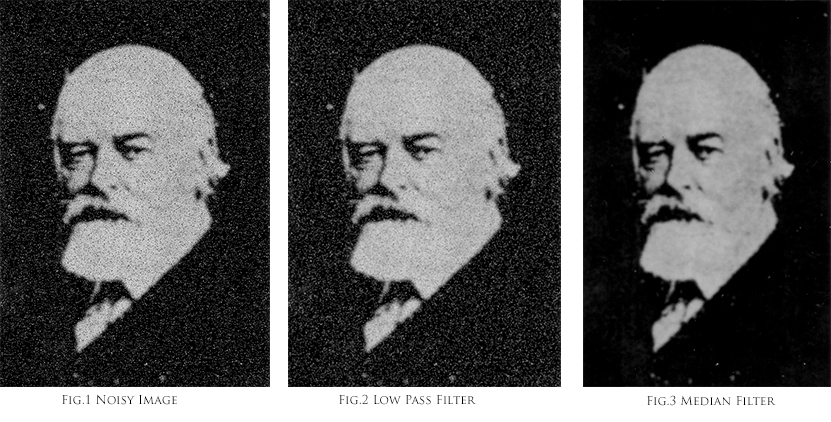
\includegraphics[width=80mm]{output1.jpg}
	\captionof{figure}{Direct Filter
		  \label{overflow}}
\end{minipage} 

\begin{minipage}{\linewidth}
	\centering
	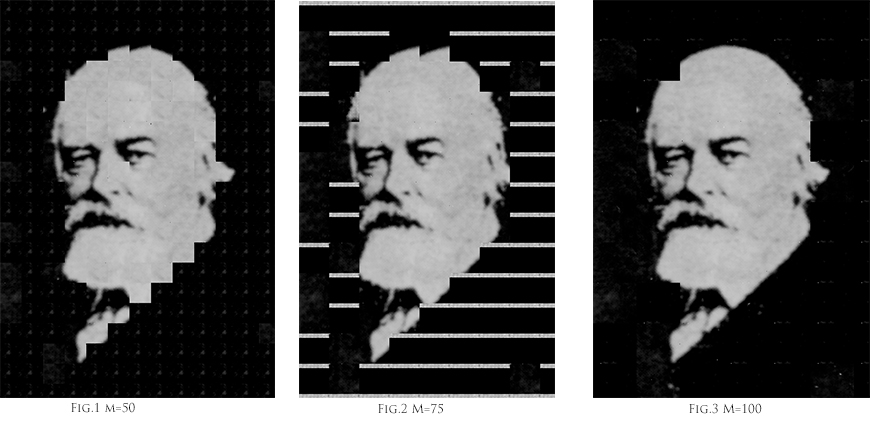
\includegraphics[width=80mm]{output2.jpg}
	\captionof{figure}{Dictionary Based Filter for m=50,75,100
		\label{overflow}}
\end{minipage} 

We can infer form the output that median filters are much more accurate than low pass filter for image with salt and pepper noise.


\begin{minipage}{\linewidth}
	\centering
	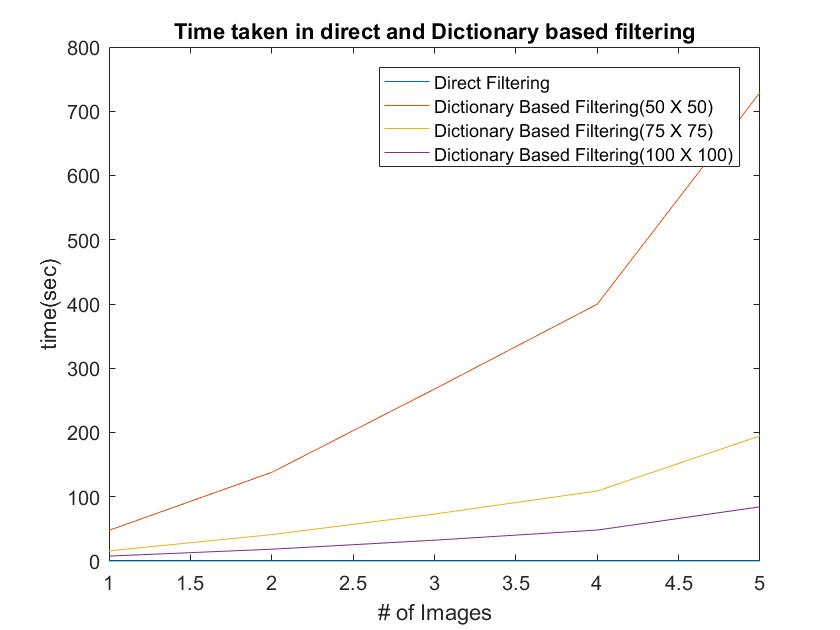
\includegraphics[width=80mm]{Timeanalysis.jpg}
	\captionof{figure}{Time Analysis
		\label{overflow}}
\end{minipage} 

Above analysis states that less the value of m more is the time taken to filter images. This is mainly due to size of dictionary. Less is the value of m, more is value of threshold and more is value of dictionary. It would take more time to search in a big dictionary. Here, time is exponentially varying with no. of images.
\vspace{0.5cm}
\begin{center}
	\begin{tabular}{||c c c ||} 
	\hline
	Dimension(m) & Threshold  & Percentage Error \\ 
	\hline\hline
	50 x 50 & 175 & 9.89 \%  \\ 
	\hline
	75 x 75 & 140 & 9.19 \% \\ 
	\hline
	100 x 100 & 90  & 3.5 \% \\ 
	
\end{tabular}\\
 \small Table-1 Error Analysis 
\end{center}
Here, more is the value of m, less is the percentage error.


	
	\ifCLASSOPTIONcaptionsoff
	\newpage
	\fi
	
\section{\textbf{Conclusion}}
	While using dictionary based filtering for median filter we can conclude that more is the value of m, better is the performance. Direct approach is much more efficient than dictionary based approach for median filter for lower no. of images. Dictionary based approach can be used with filters with higher polynomial terms. 
	
    \section{\textbf{Future Work}}
    We would try to implement more efficient searching algorithm to search image from the dictionary and try the whole approach of dictionary based filtering for filters with higher polynomial terms.
	
	
	\begin{thebibliography}{8}
	\bibitem{IEEEhowto:kopka}
	"K-SVD", En.wikipedia.org, 2017. [Online]. Available: \url{https://en.wikipedia.org/wiki/K-SVD}. [Accessed: 03- Mar- 2017].	\bibitem{IEEEhowto:kopka}
	"Sparse dictionary learning", En.wikipedia.org, 2017. [Online]. Available:\url{https://en.wikipedia.org/wiki/Sparse_dictionary_learning}	[Accessed: 25- Feb- 2017].
	\bibitem{IEEEhowto:kopka}
	A.  Rosebrock, "Convolutions with OpenCV and Python - PyImageSearch", PyImageSearch, 2017. [Online]. Available:\url{ http://www.pyimagesearch.com/2016/07/25/convolutions-with-opencv-and-python/}. [Accessed: 01- Mar- 2017].
	
	\bibitem{IEEEhowto:kopka}"on-line dictionary Learning",\url{https://en.wikipedia.org/wiki/Sparse_dictionary_learning#Online_dictionary_learning}.[Accessed: 06- Mar- 2017]
	
	\bibitem{IEEEhowto:kopka}
	"How to Split Image Into Multiple Pieces in Python", Stackoverflow.com, 2017. [Online]. Available: \url{http://stackoverflow.com/questions/5953373/how-to-split-image-into-multiple-pieces-in-python}. [Accessed: 01- Mar- 2017].
	
	\bibitem{IEEEhowto:kopka}
	"Image denoising using dictionary learning — scikit-learn 0.18.1 documentation", Scikit-learn.org, 2017. [Online]. Available: \url{http://scikit-learn.org/stable/auto_examples/decomposition/plot_image_denoising.html}. [Accessed: 01- Mar- 2017].
	
	\bibitem{IEEEhowto:kopka}
	"Result of On-line Dictionary Learning for m=2,4,8,12,16",\url{https://github.com/kitsune-udon/online_dictionary_learning}.[Accessed: 02- April- 2017]
	\bibitem{IEEEhowto:kopka}
	Lijun Xu, "A Study of the K-SVD Algorithm for Designing Overcomplete Dictionaries for Sparse Representation" [Source:unknown]. [Accessed: 06- May- 2017]
	\bibitem{IEEEhowto:kopka}
	“Digital Image Processing”, JAYARAMAN
	\bibitem{IEEEhowto:kopka}
	"Median filter", En.wikipedia.org, 2017. [Online]. Available: \url{https://en.wikipedia.org/wiki/Median_filter}. [Accessed: 03- Mar- 2017].
	\bibitem{IEEEhowto:kopka}
	Michal Aharon, Michael Elad, and Alfred Bruckstein,"K-SVD: An Algorithm for Designing Overcomplete Dictionaries for Sparse Representation",Publication: IEEE TRANSACTIONS ON SIGNAL PROCESSING, VOL. 54, NO. 11, NOVEMBER 2006.[Accessed on: 21- Mar- 2017]
	\bibitem{IEEEhowto:kopka}
	"Result of K-SVD",\url{https://github.com/alsoltani/K-SVD}
	
	
		
	\end{thebibliography}
	
	
	
\end{document}


